\section{Oscillators}
\subsection{Oscillation Condition}
\begin{itemize}
    \itemsep0pt
    \item Oscillation condition:
        \begin{align*}
            &|k| \cdot |V_u| = 1, \quad V_u = \dfrac{U_v}{U_e}, k = \dfrac{U_a}{U_v}\\
            &\varphi_v + \varphi_k = 0\text{ or }n\,2\pi
        \end{align*}
    \item Classification by feedback principle:
    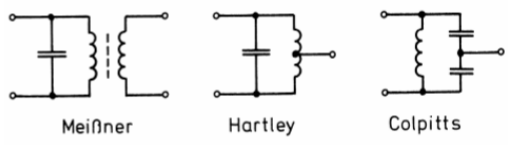
\includegraphics[width=7.5cm]{content/hfcomp/pictures/oscillator_types.png}
\end{itemize}
\subsection{Variable Oscillators}
\begin{itemize}
    \itemsep0pt
    \item Colpitts common base circuit:
        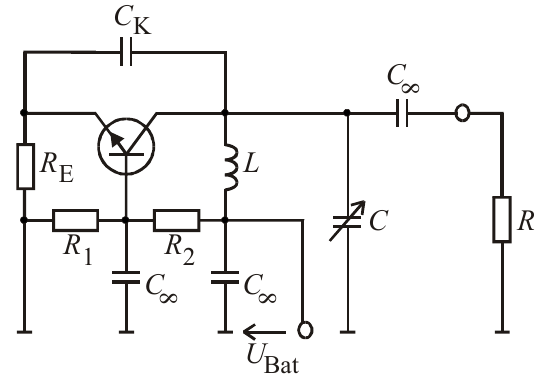
\includegraphics[width=6.5cm]{content/hfcomp/pictures/colpitts_bipolar_common_base_oscillator.png}
        \begin{align*}
            &f_S = f_T: \to \alpha \approx -\dfrac{j}{\sqrt{2}}\\
            &\omega_S C_K Z_K = \dfrac{1}{j\alpha} = \sqrt{2}
        \end{align*}
%    \item General oscillator circuit with transistor (Bipolar or FET):
%        \begin{equation*}
%            \rotatebox{-90}{%
%            $\begin{bmatrix}
%                (Y_1 + Y_3 + Y_i) & -(Y_1 + Y_i) & -Y_3 & 0\\
%                -(Y_1 + Y_i + g_m) & (Y_1 + Y_2 + Y_i + Y_0 + g_m) & -Y_2 & -Y_0\\
%                -Y_3 & -Y_2 & (Y_2 + Y_3) & 0\\
%                g_m & -(Y_0 + g_m) & 0 & Y_0
%            \end{bmatrix}
%            \begin{bmatrix}
%                U_1\\
%                U_2\\
%                U_3\\
%                U_4
%            \end{bmatrix}
%            =0
%            $}
%        \end{equation*}
\end{itemize}
\subsection{Quarz-Oscillators}
\begin{itemize}
    \itemsep0pt
    \item Oscillator stability: $\dfrac{10^{-4}}{K},\dfrac{10^{-6}}{K}...\dfrac{10^{-9}}{K}$
    \item Piezo-electric oscillator: \textit{thickness oscillator}
\end{itemize}
\begin{circuitikz}[
        scale=.9,
        transform shape]
    % ECD
    \draw (0,0) to[short, o-*] (1,0) (1,1) to[short] (1,-1);
    \draw (1,1) to[L=$L_S$, american] (3,1) to[C=$C_S$] (5,1) to[R=$R_S$] (7,1) -- (7,-1);
    \draw (1,-1) to[C=$C_p$] (7,-1);
    \draw (7,0) to[short, *-o] (8,0);
    % Labels
    \draw (.5,1.8)node[]{{\large \textbf{ECD:}}};
    \draw (.8,-1.4) to[out=270, in=180] (1,-1.6) -- (3.8, -1.6) -- (4, -1.8)node[below]{$jX$} -- (4.2, -1.6) -- (7,-1.6) to[out=0, in=270] (7.2,-1.4); 
\end{circuitikz}

\subsection{Mixer, Phase Detector}
\begin{itemize}
    \item Mixing gain (loss):
        \begin{equation*}
            g_M = 10 \lg\dfrac{P_a}{P_{1,\mathrm{max}}}
        \end{equation*}
\end{itemize}
\subsection{PLL-Circuit (Phase Locked Loop)}
\begin{itemize}
    \itemsep0pt
    \item Phase of the output signal of a controllable oscillator is locked to the phase of a reference signal by a feedback loop
    \begin{tikzpicture}[
        block/.style={
            draw,
            rectangle,
            minimum size = 1cm,
            thick,
            text centered
        },
        generator/.style={
            draw,
            circle,
            minimum size = 1cm,
            thick,
            text centered
        },
        >=Stealth,
        scale=.9,
        transform shape
    ]
    % VCO
    \node [generator](VCO) at (0,0){VCO};
    % Frequency divider 1/n
    \node[block](n) at (3,0){};
    \draw (n.south west) -- (n.north east);
    \node[above left] at (n.center){$n$};
    \node[below right] at (n.center){$1$};
    % Phase Discriminator
    \node[block](PD) at (6,0){$\varphi$};
    % Frequency Divider 1/m
    \node[block](m) at (6,2){};
    \draw (m.south west) -- (m.north east);
    \node[above left] at (m.center){$m$};
    \node[below right] at (m.center){$1$};
    % Local Oscillator
    \node[generator](LO) at (3,2){LO};
    % Lowpass Filter
    \node[block](LP) at (4.5,-2){LP};
    % Inverter
    \node[block](inv) at (1.5,-2){-1};

    % Control Loop Arrows
    \draw[->] (VCO.east) --node[below](out){} (n.west);
    \draw[->] (n.east) --node[above]{$f_0/n$} (PD.west);
    \draw[->] (PD.south) |-node[right, pos=.2]{$-U_{DC}$} (LP.east);
    \draw[->] (LP.west) -- (inv.east);
    \draw[->] (inv.west) -|node[left, pos=.75]{$U_{DC}$} (VCO.south);
    % Output Arrow
    \draw[->] (out) --node[left]{$f_0$} ++(0,1.5);
    % Reference Signal Arrows
    \draw[->] (LO.east) --node[above]{$f_Q$} (m.west);
    \draw[->] (m.south) --node[right]{$f_Q/m$} (PD.north);
\end{tikzpicture}

    \begin{equation*}
        f_0 = \dfrac{n}{m} f_Q
    \end{equation*}
    \item Digital frequency detection and division
\end{itemize}
\subsection{Two-Terminal-(1-Port)-Oscillators}
\begin{equation*}
    \text{Stability:} \dfrac{\partial Y_k}{\partial\sigma} > 0
\end{equation*}
\subsection{Oscillator Noise}
Leeson's Model for Oscillator Phase Noise:\\
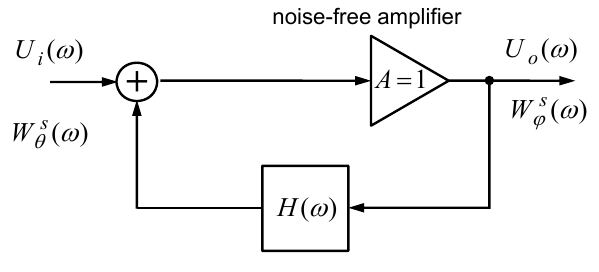
\includegraphics[width=.3\paperheight]{content/hfcomp/pictures/leeson_model_phase_noise.png}
